\input{../utils/slide-preamble.tex}
\input{../utils/color-palettes.tex}
\input{../utils/dpp-preamble.tex}
\input{../utils/macros.tex}
\begin{table}[htbp]
    \sffamily
    \small
    \rowcolors{2}{}{mygray}
    \addtolength{\tabcolsep}{-0.1cm}
\caption{
    A key to some of the notation used in the text.
}
    \centering
    \begin{tabular}{ l >{\raggedright\hangindent=0.5cm}m{14cm} }
        \toprule
        \textbf{Symbol} & \textbf{Description} \tn
        \midrule
        \ncomparisons{} & The number of population pairs being compared.
        \tn
        \nevents{} & The number of divergence times (or ``events'') across the
            population pairs being compared.
        \tn
        \comparisondivtime[i] & The time in the past when the two populations
            of pair $i$ diverged.
        \tn
        \divtime & The time of a divergence event at which one or more pairs of
            populations diverged.
        \tn
        \divtimemodel & The divergence model, which comprises the divergence
            times and the mapping of the population pairs to those times.
        \tn
        \divtimes & All of the unique divergence times in the model
            ($\divtimes = \divtime[1], \ldots, \divtime[\nevents]$).
        \tn
        \divtimesets & The mapping of population pairs to divergence events,
            but not the times of the events.
        \tn
        \basedistribution & The base distribution of the Dirichlet process.
        \tn
        \concentration & The concentration parameter of the Dirichlet process.
        \tn
        \allelecount, \redallelecount & The number of copies of a locus sampled
            from a population, and the number of those copies that are the ``red''
            allele.
            \tn
        \leafallelecounts, \leafredallelecounts & The allele counts from both
            populations of a pair (i.e., $\leafallelecounts, \leafredallelecounts =
            (\allelecount[1], \redallelecount[1]), 
            (\allelecount[2], \redallelecount[2])$).
            \tn
        \comparisondata[i] & The allele counts across all the loci from
            population pair $i$. I.e., all of the characters being analyzed for
            population pair $i$.
            \tn
        \nloci & The number of loci collected for a pair of populations.
        \tn
        \alldata & All of the data being analyzed, i.e., the
            character matrices from all population pairs.
        \tn
        \genetree & A gene tree with branch lengths.
        \tn
        \murate & The rate of mutation.
        \tn
        \rgmurate & Relative rate of mutating from the ``red'' to ``green'' state.
        \tn
        \grmurate & Relative rate of mutating from the ``green'' to ``red'' state.
        \tn
        \gfreq & The stationary frequency of the ``green'' state.
        \tn
        \epopsize[\rootpopindex] & The effective size of the ancestral population.
        \tn
        \epopsize[\descendantpopindex{1}], \epopsize[\descendantpopindex{2}] &
            The effective sizes of the two descendant populations of a pair.
        \tn
        \comparisonpopsizes & Shorthand notation for all three effective
            population sizes for a pair (ancestral and the two descendant
            populations).
        \tn
        \sptree & The species tree for a pair of populations. This comprises the
            three effective population sizes (ancestral and the two descendant)
            and the time of divergence.
            \tn
        \bottomrule
    \end{tabular}
    \label{table:notation}
\end{table}


\input{../utils/slide-macros.tex}
\bibliography{../bib/references}

\title[Ecoevolity workshop]{SSB 2018 Comparative Phylogeography Workshop}

\author[Jamie Oaks]{
    Jamie R.\ Oaks}

\institute[\href{http://phyletica.org}{phyletica.org}]{
    % \inst{1}%
    Department of Biological Sciences \&
    % \inst{2}
    Museum of Natural History,
    Auburn University
}

% \date{\today}
\date{June 4, 2018}


\setbeamersize{text margin left=3mm, text margin right=3mm}

\begin{document}

% \maketitle

\begin{frame}
    \begin{columns}

        \column{.49\textwidth}

        \vspace{-2cm}
        \begin{minipage}[c][\headlessframetextheight][c]{0.98\columnwidth}
            \maketitle
        \end{minipage}

        \column{.49\textwidth}

        \begin{minipage}[t][\headlessframetextheight][c]{\columnwidth}
            \begin{figure}
                \begin{center}
                    \smartgraphic[\headlessframetextheight]{}{../images/darwin-tol-copyright-boris-kulikov-2007.jpg}
                \vspace{-2.0mm}
                \caption{\tiny \copyright~2007 Boris Kulikov \href{http://boris-kulikov.blogspot.com/}{boris-kulikov.blogspot.com}}
                \end{center}
            \end{figure}
        \end{minipage}
    \end{columns}
\end{frame}



% \input{intro-general.tex}

% \input{intro-shared-divs.tex}

% \input{shared-div-example-long.tex}
\input{shared-div-example-medium.tex}

\begin{frame}[c,label=violations]
    % \frametitle{Violations are pervasive and interesting}
    % \frametitle{Shared divergences are pervasive and interesting}

    \begin{columns}

        \column{0.52\textwidth}

        \begin{minipage}[c][\frametextheight][c]{0.95\columnwidth}
            \raggedright
            \uncover<1->{
            Biogeography
            \begin{itemize}
                \item Environmental changes that affect whole communities of species
            \end{itemize}
            }

            \uncover<2->{
            Gene family evolution
            \begin{itemize}
                \item Chromosomal duplications
            \end{itemize}
            }

            \uncover<3->{
            Epidemiology
            \begin{itemize}
                \item Disease spread via co-infected individuals
                \item Transmission at social gatherings
            \end{itemize}
            }

            \uncover<4->{
            Endosymbiont evolution (e.g., parasites, microbiome)
            \begin{itemize}
                \item Speciation of the host
                \item Co-colonization of new host species
            \end{itemize}
            }
        \end{minipage}

        \column{0.46\textwidth}

        \begin{minipage}[c][\contentheight][c]{\columnwidth}
            \centering
            % \resizebox{!}{0.75\frametextheight}{%
            \resizebox{!}{0.71\frametextheight}{%
                \input{shared-div-tree.tex}
            }
        \end{minipage}
    \end{columns}

\end{frame}

\begin{frame}<handout:0|beamer:0>[noframenumbering,label=whycare]
    \frametitle{Why account for shared divergences?}

    \begin{enumerate}
        \item<2-> Improve inference
        \vspace{3mm}
        \item<3-> \textbf{Provide a framework for studying processes of
                co-diversification}
    \end{enumerate}

\end{frame}

\againframe<1-2>{whycare}

% \input{shared-div-advantages.tex}
\input{shared-div-advantages-bare.tex}

\againframe<2->{whycare}

\againframe<4->{violations}


\input{shared-div-example-very-short.tex}

\input{div-model-cartoons.tex}
    
\input{div-model-choice.tex}

\begin{frame}

    \begin{itemize}
        \item<1-> Let's assume we are interested in the probability of a coin we
            have not seen landing heads-side up when it is flipped
            (\probheads)

        \item<2-> Before flipping, we decide to compare two models that vary in our
            prior assumptions about the probability of the coin landing heads
            up

        \item<3-> We assume:
        \begin{enumerate}
            \item The coin is probably fair \\

                \vspace{1.0ex}
                \coinmodel[1]: $\probheads \sim \textrm{Beta}(5.0, 5.0)$

            \vspace{2ex}
            \item the coin is weighted to land tails side up most of time \\

                \vspace{1.0ex}
                \coinmodel[2]: $\probheads \sim \textrm{Beta}(1.0, 5.0)$
        \end{enumerate}
    \end{itemize}
\end{frame}


\begin{frame}
    \begin{itemize}
        \item<1-> We do 100 flips and 50 land heads up

        \item<2-> Now, we can calculate the posterior distribution for
            the probability of landing heads up under both our models
    \end{itemize}

    \onslide<3->{
    \begin{displaybox}[0.60\linewidth]
        \[
            p(\probheads \given \flipdata, \coinmodel[i]) = \frac{
                p(\flipdata \given \probheads, \coinmodel[i]) p(\probheads \given \coinmodel[i])
            }{
                p(\flipdata \given \coinmodel[i])
            }
        \]
    \end{displaybox}
    }

    \begin{itemize}
        \item<4-> We see the posterior distribution of \probheads is very
            robust to our prior assumptions

        \item<4-> \href{https://kerrycobb.github.io/beta-binomial-web-demo/}{https://kerrycobb.github.io/beta-binomial-web-demo/}
    \end{itemize}
\end{frame}


\begin{frame}
    \begin{itemize}
        \item<1-> However, we want to compare the ability of the models to explain the
            data
        \item<2-> We need to average (integrate) the likelihood density function
            over all possible values of \probheads, weighting by the prior
    \end{itemize}

    \onslide<3->{
    \begin{displaybox}[0.60\linewidth]
        \vspace{-2ex}
        \[
            p(\flipdata \given \coinmodel[1]) =
            \int_{\probheads}
            p( \flipdata \given \probheads, \coinmodel[1])
            p(\probheads \given \coinmodel[1])
            \diff{\probheads}
        \]
    \end{displaybox}
    }
\end{frame}


\begin{frame}
    \begin{itemize}
        \item<1-> Why do we care about the marginal likelihood?
        \item<2-> It's \emph{the evidence} that updates our prior to give us
            the posterior probability of the model
    \end{itemize}

    \onslide<3->{
    \begin{displaybox}[0.80\linewidth]
        \vspace{0.7ex}
        \[
            p(\coinmodel[1] \given \flipdata) = \frac{
                p(\flipdata \given \coinmodel[1])
                p(\coinmodel[1])
            }{
                p(\flipdata \given \coinmodel[1])
                p(\coinmodel[1])
                +
                p(\flipdata \given \coinmodel[2])
                p(\coinmodel[2])
            }
        \]
        \vspace{0ex}
    \end{displaybox}
    }
\end{frame}


\begin{frame}[t]
    % \frametitle{Causes of bias: Marginal likelihoods}
    % \frametitle{Causes of bias: Broad priors}
    ``Bad'' priors on div times can lead to poor marginal likelihoods for
    models with more div-time parameters
    \begin{displaybox}[5.5cm]
        \small
        \[
            p(X) = \int_{\theta} p(X
            \given \theta) p(\theta) \mathrm{d}\theta
        \]%\vspace{0mm}
    \end{displaybox}
    \smallskip
    \centerline{
        % \includegraphics<2>[height=6.5cm]{../images/marginal-plot-2d-no-priors.pdf}
        \includegraphics<1>[height=6.5cm]{../images/marginal-plot-2d-uniform-prior.pdf}
        % \includegraphics<3>[height=6.5cm]{images/marginal-plot-2d.pdf}
    }
\end{frame}

\begin{frame}
    % \frametitle{Causes of bias: Marginal likelihoods}
    ``Bad'' priors on div times can lead to poor marginal likelihoods for
    models with more div-time parameters
    % \begin{displaybox}[5.5cm]
    %     \small
    %     \[
    %         p(X) = \int_{\theta} p(X
    %         \given \theta) p(\theta) \mathrm{d}\theta
    %     \]%\vspace{0mm}
    % \end{displaybox}
    % \smallskip
    \centerline{
        % \includegraphics<1>[height=8.0cm]{../images/marginal-plot-3d-bare.png}
        % \includegraphics<2>[height=8.0cm]{../images/marginal-plot-3d-prior.png}
        \includegraphics<1>[height=8.0cm]{../images/marginal-plot-3d.png}}
\end{frame}


\againframe<7->{fullmodel}

\begin{frame}
    \begin{center}
        \LARGE
        \href{https://github.com/phyletica/ecoevolity}{
            \textbf{\textcolor{pgreen}{E}\textcolor{pteal}{co\textcolor{pauburn}{evo}lity}}}:
        \textcolor{pgreen}{\bf E}stimating \textcolor{pauburn}{\bf evo}lutionary \textcolor{pteal}{\bf coevality}
    \end{center}

    \begin{itemize}
        \item<2-> CTMC model of characters evolving along genealogies
        \item<2-> Coalescent model of genealogies branching within populations
        \item<2-> Dirichlet-process prior across divergence models
        \item<2-> Gibbs sampling\footnote{\tiny\shortfullcite{Neal2000}}
                  to numerically sample models
        \item<2-> Analytically integrate over genealogies\footnote{\tiny\shortfullcite{Bryant2012}}

        \bigskip
        \item<3-> \textsl{Goal: Fast, full-likelihood Bayesian method to infer
                patterns of co-diversification from genome-scale data}
    \end{itemize}
\end{frame}


% \input{paic-study.tex}

% \begin{frame}[t,label=challenges]
    \frametitle{Approach \#1}

    \textbf{Challenges:} \\
    \begin{minipage}[t][0.35\textheight][t]{\linewidth}
    \begin{enumerate}
        % \item<8-> Cannot solve all the integrals analytically
        \item<1-> Likelihood is tractable, but difficult
        \begin{itemize}
            \item<2-> Use an existing method!
        \end{itemize}
        % \begin{itemize}
        %     \item<2-> Numerical approximation via approximate-likelihood Bayesian computation (ABC)
        % \end{itemize}
    \end{enumerate}
    \end{minipage}

    \begin{minipage}[t][0.35\textheight][t]{\linewidth}
    \begin{enumerate}
        \setcounter{enumi}{1}
        \item<1-> Sampling over all possible models
        \begin{itemize}
            % \item<3-> A ``diffuse'' Dirichlet process prior (DPP)
            \item<2-> Use an existing method! 
        \end{itemize}
    \end{enumerate}
    \end{minipage}
    % \barefootnote{\tiny \shortfullcite{Oaks2012}, \shortfullcite{Oaks2014dpp}}
\end{frame}


% \begin{frame}[t]
    \vspace{-5mm}
    \begin{center}
    \smartgraphic{<1>}{../images/old-paic-results/negros-panay-msbayes.pdf}
    \end{center}
    \barefootnote{\shortfullcite{Oaks2012}}
\end{frame}


% \begin{frame}<handout:0|beamer:0>[t,noframenumbering,label=approach2]
    \frametitle{Approach \#2}

    \textbf{Challenges:} \\
    \begin{minipage}[t][0.35\textheight][t]{\linewidth}
    \begin{enumerate}
        % \item<8-> Cannot solve all the integrals analytically
        \item<1-> Likelihood is tractable, but difficult
        % \begin{itemize}
        %     \item<2-> Use an existing method!
        % \end{itemize}
        \begin{itemize}
            \item<2-> Numerical approximation via approximate-likelihood Bayesian computation (ABC)
        \end{itemize}
    \end{enumerate}
    \end{minipage}

    \begin{minipage}[t][0.35\textheight][t]{\linewidth}
    \begin{enumerate}
        \setcounter{enumi}{1}
        \item<1-> Sampling over all possible models
        \begin{itemize}
            \item<3-> A ``diffuse'' Dirichlet process prior (DPP)
            % \item<2-> Use an existing method! 
        \end{itemize}
    \end{enumerate}
    \end{minipage}
    % \barefootnote{\tiny \shortfullcite{Oaks2012}, \shortfullcite{Oaks2014dpp}}
\end{frame}

\againframe<1-2>{approach2}

\blankslide

\againframe<2->{approach2}


% \begin{frame}
\setbeamercovered{invisible}

% Set the overall layout of the tree
\tikzstyle{level 1}=[level distance=8em, sibling distance=10.8em]
\tikzstyle{level 2}=[level distance=11em, sibling distance=4.3em]

% Define styles
\tikzstyle{root} = [minimum width=12mm, minimum height=8mm]
\tikzstyle{internal} = [minimum width=12mm, minimum height=8mm]
\tikzstyle{tip} = [minimum width=12mm, minimum height=8mm]
\tikzstyle{branch} = [->, very thick]

\vspace{-2mm}
\uncover<6->{
\hspace{0.43\textwidth}
    {\LARGE $\boldsymbol{\alpha =} \only<6>{\mathbf{\conc}}\only<7->{\mathbf{\cconc}}$} \\
}

\vspace{4mm}

\hspace{1.2cm}
% \resizebox{!}{1.02\frametextheight}{%
\resizebox{!}{0.98\frametextheight}{%
\begin{tikzpicture}[grow=right]%, sloped]
\pgfkeys{/pgf/number format/.cd,fixed,fixed zerofill,precision=3}
\node[root] {\pgftext{\includegraphics[width=8mm]{../images/dpp-nodes/dpp-node-1.pdf}}}
    child [visible on=<2->]{
        node[internal] {\pgftext{\includegraphics[width=8mm]{../images/dpp-nodes/dpp-node-12.pdf}}}        
            child [visible on=<4->]{
                node[tip, label=right:
                    {\tiplabel{\uncover<5->{
                        $
                        % p(m = 123)=
                        \left(\frac{\alpha}{\alpha+1}\right)\left(\frac{\alpha}{\alpha+2}\right)
                        \only<6>{= \calcprob{\conc}{\conc}}
                        \uncover<7->{= \ccalcprob{\cconc}{\cconc}}$
                        }}}]
                    {\pgftext{\includegraphics[width=8mm]{../images/dpp-nodes/dpp-node-123.pdf}}}
                edge from parent [style = branch]
                node[above,
                    label={[label distance = -0.7em]\branchlabel{$\alpha$}}%$\frac{\alpha}}{\alpha+2}$}}
                    ] {}
            }
            child [visible on=<4->]{
                node[tip, label=right:
                    {\tiplabel{\uncover<5->{
                        $
                        % p(m = 121)=
                        \left(\frac{\alpha}{\alpha+1}\right)\left(\frac{1}{\alpha+2}\right)
                        \only<6>{= \calcprob{\conc}{1}}
                        \uncover<7->{= \ccalcprob{\cconc}{1}}$
                        }}}]
                    {\pgftext{\includegraphics[width=8mm]{../images/dpp-nodes/dpp-node-122.pdf}}}
                edge from parent [style = branch]
                node[above,
                    label={[label distance = -0.7em]\branchlabel{$1$}}%$\frac{1}{\alpha+2}$}}
                    ] {}
            }
            child [visible on=<4->]{
                node[tip, label=right:
                    {\tiplabel{\uncover<5->{
                        $
                        % p(m = 122)=
                        \left(\frac{\alpha}{\alpha+1}\right)\left(\frac{1}{\alpha+2}\right)
                        \only<6>{= \calcprob{\conc}{1}}
                        \uncover<7->{= \ccalcprob{\cconc}{1}}$
                        }}}]
                    {\pgftext{\includegraphics[width=8mm]{../images/dpp-nodes/dpp-node-121.pdf}}}
                edge from parent [style = branch]
                node[above,
                    label={[label distance = -0.5em]\branchlabel{$1$}}%$\frac{1}{\alpha+2}$}}
                    ] {}
            }
            edge from parent [style = branch]
            node[above,
                label={[label distance = 0em]\branchlabel{$\alpha$}}%$\frac{\alpha}{\alpha+1}$}}
                ] {}
    }
    child [visible on=<2->]{
        node[internal] {\pgftext{\includegraphics[width=8mm]{../images/dpp-nodes/dpp-node-11.pdf}}}        
            child [visible on=<3->]{
                node[tip, label=right:
                    {\tiplabel{\uncover<5->{
                        $
                        % p(m = 112)=
                        \left(\frac{1}{\alpha+1}\right)\left(\frac{\alpha}{\alpha+2}\right)
                        \only<6>{= \calcprob{1}{\conc}}
                        \uncover<7->{= \ccalcprob{1}{\cconc}}$
                        }}}]
                    {\pgftext{\includegraphics[width=8mm]{../images/dpp-nodes/dpp-node-112.pdf}}}
                edge from parent [style = branch]
                node[above,
                    label={[label distance = -0.7em]\branchlabel{$\alpha$}}%$\frac{\alpha}{\alpha+2}$}}
                    ] {}
            }
            child [visible on=<3->]{
                node[tip, label=right:
                    {\tiplabel{\uncover<5->{
                        $
                        % p(m = 111)=
                        \left(\frac{1}{\alpha+1}\right)\left(\frac{2}{\alpha+2}\right)
                        \only<6>{= \calcprob{1}{2}}
                        \uncover<7->{= \ccalcprob{1}{2}}$
                        }}}]
                    {\pgftext{\includegraphics[width=8mm]{../images/dpp-nodes/dpp-node-111.pdf}}}
                edge from parent [style = branch]
                node[above,
                    label={[label distance = -0.7em]\branchlabel{$2$}}%$\frac{2}{\alpha+2}$}}
                    ] {}
            }
            edge from parent [style = branch]
            node[above,
                label={[label distance = 0em]\branchlabel{$1$}}%$\frac{1}{\alpha+1}$}}
                ] {}
    };
\end{tikzpicture}
}

\end{frame}



% \begin{frame}<handout:0|beamer:0>[t,noframenumbering,label=approach2]
    \frametitle{Approach \#2}

    \textbf{Challenges:} \\
    \begin{minipage}[t][0.35\textheight][t]{\linewidth}
    \begin{enumerate}
        % \item<8-> Cannot solve all the integrals analytically
        \item<1-> Likelihood is tractable, but difficult
        % \begin{itemize}
        %     \item<2-> Use an existing method!
        % \end{itemize}
        \begin{itemize}
            \item<2-> Numerical approximation via approximate-likelihood Bayesian computation (ABC)
        \end{itemize}
    \end{enumerate}
    \end{minipage}

    \begin{minipage}[t][0.35\textheight][t]{\linewidth}
    \begin{enumerate}
        \setcounter{enumi}{1}
        \item<1-> Sampling over all possible models
        \begin{itemize}
            \item<3-> A ``diffuse'' Dirichlet process prior (DPP)
            % \item<2-> Use an existing method! 
        \end{itemize}
    \end{enumerate}
    \end{minipage}
    % \barefootnote{\tiny \shortfullcite{Oaks2012}, \shortfullcite{Oaks2014dpp}}
\end{frame}

\againframe<1-2>{approach2}

\blankslide

\againframe<2->{approach2}


% \input{abc.tex}

% \blankslide

% \againframe<15->{fullmodel}

% \begin{frame}
    \frametitle{New method: \dppmsbayes}
    \begin{itemize}[<+->]
        \item Approximate-likelihood Bayesian approach to inferring models of
            shared divergences
        \item Flexible Dirichlet-process prior (DPP) over all possible
            divergence models
        \item Flexible priors on parameters to avoid strongly weighted
            posteriors
        \item Multi-processing to accommodate genomic datasets
    \end{itemize}
    \barefootnote{\shortfullcite{Oaks2014dpp}}
\end{frame}


% \begin{frame}[t]
    \vspace{-5mm}
    \begin{center}
    \smartgraphic{<1>}{../images/old-paic-results/negros-panay-dpp-msbayes.pdf}

    \smartgraphic{<2>}{../images/old-paic-results/negros-panay-dpp-msbayes-sumtimes.pdf}
    \end{center}
    \barefootnote{\shortfullcite{Oaks2012}}
\end{frame}


% \input{approach-3-challenges.tex}

\begin{frame}[t]
    \frametitle{Sampling divergence models}
    \begin{uncoverenv}<2->
    \begin{itemize}
        \item The divergence models are ways of assigning our taxa to events
        \item A Dirichlet process prior (DPP) model is a convenient and flexible
            solution
            \begin{itemize}
                \item Common Bayesian approach to assigning variables to an
                    unknown number of categories
                \item Controlled by ``concentration'' parameter: $\alpha$
            \end{itemize}
    \end{itemize}

    \begin{figure}
    \begin{center}
        \includegraphics[height=0.4\textheight]{../images/peter-dirichlet.jpg}
        \caption{Peter Dirichlet}
    \end{center}
    \end{figure}
    \end{uncoverenv}
\end{frame}



\begin{frame}
\setbeamercovered{invisible}

% Set the overall layout of the tree
\tikzstyle{level 1}=[level distance=8em, sibling distance=10.8em]
\tikzstyle{level 2}=[level distance=11em, sibling distance=4.3em]

% Define styles
\tikzstyle{root} = [minimum width=12mm, minimum height=8mm]
\tikzstyle{internal} = [minimum width=12mm, minimum height=8mm]
\tikzstyle{tip} = [minimum width=12mm, minimum height=8mm]
\tikzstyle{branch} = [->, very thick]

\vspace{-2mm}
\uncover<6->{
\hspace{0.43\textwidth}
    {\LARGE $\boldsymbol{\alpha =} \only<6>{\mathbf{\conc}}\only<7->{\mathbf{\cconc}}$} \\
}

\vspace{4mm}

\hspace{1.2cm}
% \resizebox{!}{1.02\frametextheight}{%
\resizebox{!}{0.98\frametextheight}{%
\begin{tikzpicture}[grow=right]%, sloped]
\pgfkeys{/pgf/number format/.cd,fixed,fixed zerofill,precision=3}
\node[root] {\pgftext{\includegraphics[width=8mm]{../images/dpp-nodes/dpp-node-1.pdf}}}
    child [visible on=<2->]{
        node[internal] {\pgftext{\includegraphics[width=8mm]{../images/dpp-nodes/dpp-node-12.pdf}}}        
            child [visible on=<4->]{
                node[tip, label=right:
                    {\tiplabel{\uncover<5->{
                        $
                        % p(m = 123)=
                        \left(\frac{\alpha}{\alpha+1}\right)\left(\frac{\alpha}{\alpha+2}\right)
                        \only<6>{= \calcprob{\conc}{\conc}}
                        \uncover<7->{= \ccalcprob{\cconc}{\cconc}}$
                        }}}]
                    {\pgftext{\includegraphics[width=8mm]{../images/dpp-nodes/dpp-node-123.pdf}}}
                edge from parent [style = branch]
                node[above,
                    label={[label distance = -0.7em]\branchlabel{$\alpha$}}%$\frac{\alpha}}{\alpha+2}$}}
                    ] {}
            }
            child [visible on=<4->]{
                node[tip, label=right:
                    {\tiplabel{\uncover<5->{
                        $
                        % p(m = 121)=
                        \left(\frac{\alpha}{\alpha+1}\right)\left(\frac{1}{\alpha+2}\right)
                        \only<6>{= \calcprob{\conc}{1}}
                        \uncover<7->{= \ccalcprob{\cconc}{1}}$
                        }}}]
                    {\pgftext{\includegraphics[width=8mm]{../images/dpp-nodes/dpp-node-122.pdf}}}
                edge from parent [style = branch]
                node[above,
                    label={[label distance = -0.7em]\branchlabel{$1$}}%$\frac{1}{\alpha+2}$}}
                    ] {}
            }
            child [visible on=<4->]{
                node[tip, label=right:
                    {\tiplabel{\uncover<5->{
                        $
                        % p(m = 122)=
                        \left(\frac{\alpha}{\alpha+1}\right)\left(\frac{1}{\alpha+2}\right)
                        \only<6>{= \calcprob{\conc}{1}}
                        \uncover<7->{= \ccalcprob{\cconc}{1}}$
                        }}}]
                    {\pgftext{\includegraphics[width=8mm]{../images/dpp-nodes/dpp-node-121.pdf}}}
                edge from parent [style = branch]
                node[above,
                    label={[label distance = -0.5em]\branchlabel{$1$}}%$\frac{1}{\alpha+2}$}}
                    ] {}
            }
            edge from parent [style = branch]
            node[above,
                label={[label distance = 0em]\branchlabel{$\alpha$}}%$\frac{\alpha}{\alpha+1}$}}
                ] {}
    }
    child [visible on=<2->]{
        node[internal] {\pgftext{\includegraphics[width=8mm]{../images/dpp-nodes/dpp-node-11.pdf}}}        
            child [visible on=<3->]{
                node[tip, label=right:
                    {\tiplabel{\uncover<5->{
                        $
                        % p(m = 112)=
                        \left(\frac{1}{\alpha+1}\right)\left(\frac{\alpha}{\alpha+2}\right)
                        \only<6>{= \calcprob{1}{\conc}}
                        \uncover<7->{= \ccalcprob{1}{\cconc}}$
                        }}}]
                    {\pgftext{\includegraphics[width=8mm]{../images/dpp-nodes/dpp-node-112.pdf}}}
                edge from parent [style = branch]
                node[above,
                    label={[label distance = -0.7em]\branchlabel{$\alpha$}}%$\frac{\alpha}{\alpha+2}$}}
                    ] {}
            }
            child [visible on=<3->]{
                node[tip, label=right:
                    {\tiplabel{\uncover<5->{
                        $
                        % p(m = 111)=
                        \left(\frac{1}{\alpha+1}\right)\left(\frac{2}{\alpha+2}\right)
                        \only<6>{= \calcprob{1}{2}}
                        \uncover<7->{= \ccalcprob{1}{2}}$
                        }}}]
                    {\pgftext{\includegraphics[width=8mm]{../images/dpp-nodes/dpp-node-111.pdf}}}
                edge from parent [style = branch]
                node[above,
                    label={[label distance = -0.7em]\branchlabel{$2$}}%$\frac{2}{\alpha+2}$}}
                    ] {}
            }
            edge from parent [style = branch]
            node[above,
                label={[label distance = 0em]\branchlabel{$1$}}%$\frac{1}{\alpha+1}$}}
                ] {}
    };
\end{tikzpicture}
}

\end{frame}



\begin{frame}
    \begin{center}
        \url{http://phyletica.org/dpp-demo}
    \end{center}
\end{frame}

\begin{frame}[t]
    \frametitle{Pitman-Yor Process}
    \begin{uncoverenv}<2->
    \begin{itemize}
        \item A generalization of the Dirichlet process
        \item Controlled by ``concenration'' (\concentration) and ``discount''
            (\discount) parameters
        \item When $\discount = 0$, it becomes the Dirichlet process
        \item Provides more flexibility over tail behavior (Dirichlet process
            has exponential tails)
        \item Lessens the ``rich get richer'' property of the Dirichlet process
    \end{itemize}
    \end{uncoverenv}
\end{frame}



\begin{frame}
\setbeamercovered{invisible}

% Set the overall layout of the tree
\tikzstyle{level 1}=[level distance=8em, sibling distance=10.8em]
\tikzstyle{level 2}=[level distance=11em, sibling distance=4.3em]

% Define styles
\tikzstyle{root} = [minimum width=12mm, minimum height=8mm]
\tikzstyle{internal} = [minimum width=12mm, minimum height=8mm]
\tikzstyle{tip} = [minimum width=12mm, minimum height=8mm]
\tikzstyle{branch} = [->, very thick]

\vspace{-2mm}
\uncover<6->{
\hspace{0.25\textwidth}
    {\LARGE $\boldsymbol{\concentration =} \mathbf{\ccconc}$
        \hspace{0.1\textwidth}
        $\boldsymbol{\discount = } \only<6>{\mathbf{\disc}}\only<7>{\mathbf{\ddisc}}\only<8->{\mathbf{\dddisc}}$} \\
}

\vspace{4mm}

\hspace{1.2cm}
% \resizebox{!}{1.02\frametextheight}{%
\resizebox{!}{0.98\frametextheight}{%
\begin{tikzpicture}[grow=right]%, sloped]
\pgfkeys{/pgf/number format/.cd,fixed,fixed zerofill,precision=3}
\node[root] {\pgftext{\includegraphics[width=8mm]{../images/dpp-nodes/dpp-node-1.pdf}}}
    child [visible on=<2->]{
        node[internal] {\pgftext{\includegraphics[width=8mm]{../images/dpp-nodes/dpp-node-12.pdf}}}        
            child [visible on=<4->]{
                node[tip, label=right:
                    {\tiplabel{\uncover<5->{
                        $
                        % p(m = 123)=
                        \left(\frac{\concentration+\discount}{\concentration+1}\right)\left(\frac{\concentration+2\discount}{\concentration+2}\right)
                        \only<6>{= \cccalcprob{(\ccconc+\disc)}{(\ccconc+(2*\disc))}}
                        \only<7>{= \cccalcprob{(\ccconc+\ddisc)}{(\ccconc+(2*\ddisc))}}
                        \uncover<8->{= \cccalcprob{(\ccconc+\dddisc)}{(\ccconc+(2*\dddisc))}}$
                        }}}]
                    {\pgftext{\includegraphics[width=8mm]{../images/dpp-nodes/dpp-node-123.pdf}}}
                edge from parent [style = branch]
                node[above,
                    label={[label distance = -0.7em]\branchlabel{$\concentration+2\discount$}}%$\frac{\concentration}}{\concentration+2}$}}
                    ] {}
            }
            child [visible on=<4->]{
                node[tip, label=right:
                    {\tiplabel{\uncover<5->{
                        $
                        % p(m = 121)=
                        \left(\frac{\concentration+\discount}{\concentration+1}\right)\left(\frac{1-\discount}{\concentration+2}\right)
                        \only<6>{= \cccalcprob{(\ccconc+\disc)}{(1-\disc)}}
                        \only<7>{= \cccalcprob{(\ccconc+\ddisc)}{(1-\ddisc)}}
                        \uncover<8->{= \cccalcprob{(\ccconc+\dddisc)}{(1-\dddisc)}}$
                        }}}]
                    {\pgftext{\includegraphics[width=8mm]{../images/dpp-nodes/dpp-node-122.pdf}}}
                edge from parent [style = branch]
                node[above,
                    label={[label distance = -0.7em]\branchlabel{$1-\discount$}}%$\frac{1}{\concentration+2}$}}
                    ] {}
            }
            child [visible on=<4->]{
                node[tip, label=right:
                    {\tiplabel{\uncover<5->{
                        $
                        % p(m = 122)=
                        \left(\frac{\concentration+\discount}{\concentration+1}\right)\left(\frac{1-\discount}{\concentration+2}\right)
                        \only<6>{= \cccalcprob{(\ccconc+\disc)}{(1-\disc)}}
                        \only<7>{= \cccalcprob{(\ccconc+\ddisc)}{(1-\ddisc)}}
                        \uncover<8->{= \cccalcprob{(\ccconc+\dddisc)}{(1-\dddisc)}}$
                        }}}]
                    {\pgftext{\includegraphics[width=8mm]{../images/dpp-nodes/dpp-node-121.pdf}}}
                edge from parent [style = branch]
                node[above,
                    label={[label distance = -0.5em]\branchlabel{$1-\discount$}}%$\frac{1}{\concentration+2}$}}
                    ] {}
            }
            edge from parent [style = branch]
            node[above,
                label={[label distance = 0em]\branchlabel{$\concentration+\discount$}}%$\frac{\concentration}{\concentration+1}$}}
                ] {}
    }
    child [visible on=<2->]{
        node[internal] {\pgftext{\includegraphics[width=8mm]{../images/dpp-nodes/dpp-node-11.pdf}}}        
            child [visible on=<3->]{
                node[tip, label=right:
                    {\tiplabel{\uncover<5->{
                        $
                        % p(m = 112)=
                        \left(\frac{1-\discount}{\concentration+1}\right)\left(\frac{\concentration+\discount}{\concentration+2}\right)
                        \only<6>{= \cccalcprob{(1-\disc)}{(\ccconc+\disc)}}
                        \only<7>{= \cccalcprob{(1-\ddisc)}{(\ccconc+\ddisc)}}
                        \uncover<8->{= \cccalcprob{(1-\dddisc)}{(\ccconc+\dddisc)}}$
                        }}}]
                    {\pgftext{\includegraphics[width=8mm]{../images/dpp-nodes/dpp-node-112.pdf}}}
                edge from parent [style = branch]
                node[above,
                    label={[label distance = -0.7em]\branchlabel{$\concentration+\discount$}}%$\frac{\concentration}{\concentration+2}$}}
                    ] {}
            }
            child [visible on=<3->]{
                node[tip, label=right:
                    {\tiplabel{\uncover<5->{
                        $
                        % p(m = 111)=
                        \left(\frac{1-\discount}{\concentration+1}\right)\left(\frac{2-\discount}{\concentration+2}\right)
                        \only<6>{= \cccalcprob{(1-\disc)}{(2-\disc)}}
                        \only<7>{= \cccalcprob{(1-\ddisc)}{(2-\ddisc)}}
                        \uncover<8->{= \cccalcprob{(1-\dddisc)}{(2-\dddisc)}}$
                        }}}]
                    {\pgftext{\includegraphics[width=8mm]{../images/dpp-nodes/dpp-node-111.pdf}}}
                edge from parent [style = branch]
                node[above,
                    label={[label distance = -0.7em]\branchlabel{$2-\discount$}}%$\frac{2}{\concentration+2}$}}
                    ] {}
            }
            edge from parent [style = branch]
            node[above,
                label={[label distance = 0em]\branchlabel{$1-\discount$}}%$\frac{1}{\concentration+1}$}}
                ] {}
    };
\end{tikzpicture}
}

\end{frame}



\begin{frame}
    \begin{center}
        \url{http://phyletica.org/pyp-demo}
    \end{center}
\end{frame}

\begin{frame}[t]
    \frametitle{``Uniform'' prior}
    \begin{itemize}
        \item We can also assume that every possible model (every way of
            grouping the divergence times of the population pairs) is equally
            probable \emph{a priori}
        \item In addition to this, we added what we call a ``split weight,''
            which we denote as $s$
        \item We can think of $s$ in 2 ways:
            \begin{enumerate}
                \item For a given model with \nevents{} divergence time categories,
                    the relative probability of each model with $\nevents+1$
                    categories is $s$ (and the relative probability of each model with $\nevents-1$ categories
                    is $\frac{1}{s}$)
                \item During MCMC, when we propose splitting a div time category into
                    2 groups, the prior ratio of the move is $s$ (if we propose lumping
                    two categories, the prior ratio for this move is $\frac{1}{s}$)
            \end{enumerate}
    \end{itemize}
\end{frame}

\begin{frame}[t]
    \frametitle{``Uniform'' prior}
    \begin{itemize}
        \item To get a feel for the uniform prior, on the following slides we
            will look at an example with 4 pairs of populations, with 3
            different values for the split weight $s$.
        \item Some notation for the next few slides:
            \begin{description}
                \item[\ncomparisons] The number of population pairs we are comparing
                \item[\nevents] The number of div time categories
                \item[$S(\ncomparisons,\nevents)$] The number of models that
                    have \nevents{} categories (the Stirling number of the second
                    kind)
                \item[$s^{\nevents-1}$] Relative prob of each model with \nevents{}
                    categories (we rescale this to make table readable)
                \item[$s^{\nevents-1}S(\ncomparisons,\nevents)$] Relative prob
                    of entire class of models with \nevents{} categories
                \item[$p(m_i)$] The prob of \emph{each} model 
                    with \nevents{} div time categories
            \end{description}
    \end{itemize}
\end{frame}

\begin{frame}
    \frametitle{``Uniform'' prior}
\begin{center}
Split weight $s = 1.0$
\end{center}

\begin{center}
\begin{tabular}{ c c c c c }
    \nevents & $S(\ncomparisons,
                  \nevents)$     & $s^{\nevents-1}$ & $s^{\nevents-1}
                                                      S(
                                                      \ncomparisons,
                                                      \nevents)$     & $p(m_i)$ \\
    1        & 1                 & 1     & 1                 & $\frac{1}{15}$ \\
    2        & 7                 & 1     & 7                 & $\frac{1}{15}$ \\
    3        & 6                 & 1     & 6                 & $\frac{1}{15}$ \\
    4        & 1                 & 1     & 1                 & $\frac{1}{15}$ \\
             &                   &       & 15                &                \\
\end{tabular}
\end{center}
\end{frame}

\begin{frame}
    \frametitle{``Uniform'' prior}
\begin{center}
Split weight $s = 2.0$
\end{center}

\begin{center}
\begin{tabular}{ c c c c c }
    \nevents & $S(\ncomparisons,
                  \nevents)$     & $s^{\nevents-1}$ & $s^{\nevents-1}
                                                      S(
                                                      \ncomparisons,
                                                      \nevents)$     & $p(m_i)$ \\
    1        & 1                 & 1     & 1               & $\frac{1}{47}$ \\
    2        & 7                 & 2     & 14              & $\frac{2}{47}$ \\
    3        & 6                 & 4     & 24              & $\frac{4}{47}$ \\
    4        & 1                 & 8     & 8               & $\frac{8}{47}$ \\
             &                   &       & 47              &                \\
\end{tabular}
\end{center}
\end{frame}

\begin{frame}
    \frametitle{``Uniform'' prior}
\begin{center}
Split weight $s = \frac{1}{2}$
\end{center}

\begin{center}
\begin{tabular}{ c c c c c }
    \nevents & $S(\ncomparisons,
                  \nevents)$     & $s^{\nevents-1}$ & $s^{\nevents-1}
                                                      S(
                                                      \ncomparisons,
                                                      \nevents)$     & $p(m_i)$ \\
    1        & 1                 & 8     & 8               & $\frac{8}{49}$ \\
    2        & 7                 & 4     & 28              & $\frac{4}{49}$ \\
    3        & 6                 & 2     & 12              & $\frac{2}{49}$ \\
    4        & 1                 & 1     & 1               & $\frac{1}{49}$ \\
             &                   &       & 49              &                \\
\end{tabular}
\end{center}
\end{frame}


% \begin{frame}
%     \begin{center}
%         \LARGE
%         Does it work?
%     \end{center}
% \end{frame}

% \begin{frame}
    \frametitle{\dppmsbayes: Simulation-based assessment}
        \uncover<1->{
        Validation:\\

        \smallskip
        \begin{itemize}
            \item Simulate 50,000 datasets and analyze each under the same
                model
        \end{itemize}
        }

        \uncover<2->{
        \bigskip
        Robustness:\\
        \begin{itemize}
            \item Simulate datasets that violate model assumptions and analyze
                each of them
        \end{itemize}
        }

        % \uncover<3->{
        % \bigskip
        % Compared performance with previous method, \msb
        % }
\end{frame}

\begin{frame}
    \frametitle{\dppmsbayes: Validation results}
    \begin{columns}
        \column{0.49\textwidth}

        \centering{
            \smartgraphic{<1->}{../images/validation-model-choice-dpp-no-label.pdf}
        }

        \column{0.49\textwidth}

        \centering{
            \smartgraphic{<2->}{../images/validation-model-choice-dpp-uniform-no-label.pdf}
        }
    \end{columns}
    \barefootnote{\shortfullcite{Oaks2014dpp}}
\end{frame}

% \begin{frame}
%     \frametitle{\dppmsbayes: Robustness results}
%         \centering{
%             \smartgraphic{<1->}{../images/validation-model-choice-dpp-violations-horizontal.pdf}
%             }
%     \barefootnote{\shortfullcite{Oaks2014dpp}}
% \end{frame}

% \begin{frame}
%     \frametitle{\dppmsbayes: Simulation-based power analyses}
%     Does the new method have power to detect variation in divergence times?\\

%     \bigskip
%     \begin{myitemize}
%         \item<2-> Simulate datasets in which all 22 divergence times are random
%             \smallskip
%             \begin{myitemize}
%                 \item $\divTime{} \sim U(0, \,0.5 \,MGA)$
%                 \smallskip
%                 \item $\divTime{} \sim U(0, \,1.5 \,MGA)$
%                 \smallskip
%                 \item $\divTime{} \sim U(0, \,2.5 \,MGA)$
%                 \smallskip
%                 \item $\divTime{} \sim U(0, \,5.0 \,MGA)$
%                 \smallskip
%             \end{myitemize}
%         \item<2-> $MGA$ = Millions of Generations Ago

%         \item<3-> Simulate 1000 datasets for each \divTime{} distribution
%         \item<3-> Analyze all 4000 datasets with \dppmsbayes and \msb
%     \end{myitemize}
%     \barefootnote{\tiny \shortfullcite{Oaks2012}, \shortfullcite{Oaks2014dpp}}
% \end{frame}

% \begin{frame}[t]
%     \frametitle{\dppmsbayes: Power results}
%         \begin{onlyenv}<1-2>
%         \centerline{
%         \includegraphics[width=1.13\textwidth]<1-2>{images/power-psi-old-annotate-no-pp.pdf}}
%         \vspace{0mm}
%         \centerline{
%         \includegraphics[width=1.13\textwidth]<2>{images/power-psi-dpp-annotate-no-pp.pdf}}
%         \end{onlyenv}

%         \begin{onlyenv}<3->
%         \centerline{
%         \includegraphics[width=1.13\textwidth]<3->{images/power-psi-old-annotate-pp.pdf}}
%         \vspace{0mm}
%         \centerline{
%         \includegraphics[width=1.13\textwidth]<3->{images/power-psi-dpp-annotate-pp.pdf}}
%         \end{onlyenv}

%     \begin{uncoverenv}<4->
%     \begin{itemize}
%         \item Improved power to detect temporal variation across divergences
%     \end{itemize}
%     \end{uncoverenv}
%     \barefootnote{\shortfullcite{Oaks2014dpp}}
% \end{frame}

% \begin{frame}[t]
%     \frametitle{\dppmsbayes: Power results}
%         \centerline{
%         \includegraphics[width=1.13\textwidth]<1>{images/power-psi-old-annotate-no-pp.pdf}
%         \includegraphics[width=1.13\textwidth]<2->{images/power-psi-old-annotate-pp.pdf}}

%         \vspace{0mm}
%         \centerline{
%         \includegraphics[width=1.13\textwidth]<3>{images/power-psi-dpp-annotate-no-pp.pdf}
%         \includegraphics[width=1.13\textwidth]<4->{images/power-psi-dpp-annotate-pp.pdf}}

%     \begin{uncoverenv}<5->
%     \begin{itemize}
%         \item Improved power to detect temporal variation across divergences
%     \end{itemize}
%     \end{uncoverenv}
%     \barefootnote{\shortfullcite{Oaks2014dpp}}
% \end{frame}

\begin{frame}
    \frametitle{\dppmsbayes: Performance}
    \begin{itemize}
        \item<1-> New method for estimating shared evolutionary history shows:
            \begin{enumerate}
                \item<1-> Model-choice accuracy 
                \item<1-> Robustness to model violations
                \item<1-> Power to detect variation in divergence times
                \item<1-> It's fast!
            \end{enumerate}
        % \item<2-> \textbf{dpp-msbayes allows biologists to leverage comparative
        %         genomic data to infer the affects of community-scale processes
        %         on biodiversity}
        \item<2-> \textbf{A new tool for biologists to leverage comparative
                genomic data to explore processes of co-diversification}
    \end{itemize}

    \barefootnote{\shortfullcite{Oaks2014dpp}}
\end{frame}


% \section{Empirical applications}

% \begin{frame}
% \frametitle{Outline}
% \tableofcontents[currentsection,currentsubsection]
% \end{frame}

% \input{paic-study.tex}
\begin{frame}
    \frametitle{Ecoevolity: Simulation-based assessment}
    \centering{
        \smartgraphic{<1>}{../../simulations/validation/plots/root-1000-500k-div-time-scatter.pdf}
        \smartgraphic{<2>}{../../simulations/validation/plots/root-1000-500k-nevents.pdf}
        \smartgraphic{<3>}{../../simulations/validation/plots/100k-sites-est-vs-true-prob-nevent-1.pdf}
    }
\end{frame}


\begin{frame}
    % \frametitle{Ecoevolity: Simulation-based assessment}
    \centering{
        \smartgraphic{<1>}{../../simulations/validation/plots/linkage-500k-div-time-no-vo-scatter.pdf}
        \smartgraphic{<2>}{../../simulations/validation/plots/linkage-500k-nevents-no-vo.pdf}
    }
\end{frame}


% \input{msg-data.tex}

% \begin{frame}
    \frametitle{Ecoevolity: Results}
    \centering{
        \smartgraphic{<1>}{../images/ecoevolity/geckos/pyco-sumevents-cyrtodactylus-conc5-rate200-pycoevolity-nevents.pdf}
        \smartgraphic{<2>}{../images/ecoevolity/geckos/pyco-sumtimes-cyrtodactylus-conc5-rate200-pycoevolity-times.pdf}
    }
\end{frame}

\begin{frame}
    \frametitle{Our journey}
        \includegraphics<1->[width=0.32\textwidth]{../images/old-paic-results/negros-panay-msbayes.pdf}
        \includegraphics<2->[width=0.32\textwidth]{../images/old-paic-results/negros-panay-dpp-msbayes.pdf}
        \includegraphics<3->[width=0.32\textwidth]{../images/ecoevolity/geckos/pyco-sumevents-cyrtodactylus-conc5-rate200-pycoevolity-nevents.pdf}

    \begin{uncoverenv}<4->
        \begin{center}
        {\Large Conclusions?}
        \end{center}
    \end{uncoverenv}
\end{frame}


% \input{africa.tex}

% \input{empirical-conclusions.tex}

% \section{Current and future directions}

% \begin{frame}
% \frametitle{Outline}
% \tableofcontents[currentsection,currentsubsection]
% \end{frame}

% \input{full-likelihood.tex}

% \input{full-phylo.tex}



%%%%%%%%%%%%%%%%%%%%%%%%%%%%%%%%%%%%%%%%%%%%%%%%%%%%%%%%%%%%%%%%%%%%%
%%%%%%%%%%%%%%%%%%%%%%%%%%%%%%%%%%%%%%%%%%%%%%%%%%%%%%%%%%%%%%%%%%%%%
%% Marginal like coin flip example
%%%%%%%%%%%%%%%%%%%%%%%%%%%%%%%%%%%%%%%%%%%%%%%%%%%%%%%%%%%%%%%%%%%%%
%%%%%%%%%%%%%%%%%%%%%%%%%%%%%%%%%%%%%%%%%%%%%%%%%%%%%%%%%%%%%%%%%%%%%

% \begin{frame}
    \frametitle{Everything is on GitHub\ldots}
    Software:\\
    \begin{itemize}
        \item Ecoevolity:
            \url{https://github.com/phyletica/ecoevolity}

        \item PyMsBayes:
            \url{https://joaks1.github.io/PyMsBayes}

        \item dpp-msbayes:
            \url{https://github.com/joaks1/dpp-msbayes}

        \item ABACUS: Approximate BAyesian C UtilitieS.
            \url{https://github.com/joaks1/abacus}
    \end{itemize}

    \medskip
    Open-Science Notebook:\\
    \begin{itemize}
        \item Ecoevolity experiments:
            \url{https://github.com/phyletica/ecoevolity-experiments}
    \end{itemize}
    \begin{itemize}
        \item msBayes experiments:
            \url{https://github.com/joaks1/msbayes-experiments}
    \end{itemize}
\end{frame}


% \input{end-slides.tex}

% Extra slides
%%%%%%%%%%%%%%

% \begin{frame}[noframenumbering]
% \end{frame
% \begin{frame}[t]
    \frametitle{Ecoevolity: ``Bake off''}
    \centering{
        \smartgraphic{<1>}{../../bake-off/plots/divergence-time-scatter.pdf}
        \smartgraphic{<2>}{../../bake-off/plots/root-population-size-scatter.pdf}
        \smartgraphic{<3->}{../../bake-off/plots/nevents.pdf}
    }
    \begin{uncoverenv}<4->
    \begin{center}
    Average run time:
    \begin{columns}
        \column{0.32\textwidth}
        \begin{center}
        33.4 minutes
        \end{center}
        \column{0.65\textwidth}
        \begin{center}
        4.4 days
        \end{center}
    \end{columns}
    \end{center}
    \end{uncoverenv}
\end{frame}


% \begin{frame}
    \frametitle{Ecoevolity results}
\centerline{
\onslide<1->{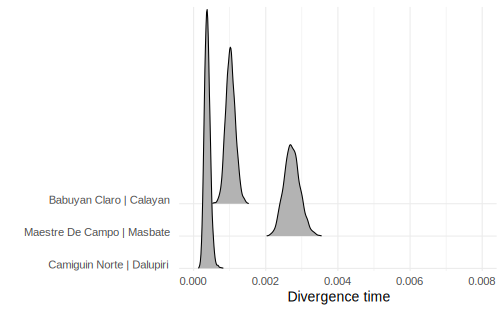
\includegraphics[height=5.4cm]{../../gekko-bake-off/results/pycoevolity-times.pdf}}
\onslide<1->{\includegraphics[height=5.4cm]{../../gekko-bake-off/results/pycoevolity-nevents.pdf}}
}

\bigskip
Run time: 7.6 minutes
\end{frame}

\begin{frame}
    \frametitle{dpp-msbayes results}
\centerline{
\onslide<1->{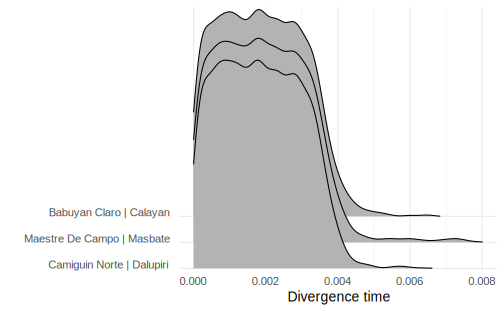
\includegraphics[height=5.4cm]{../../gekko-bake-off/results/dppmsbayes-times.pdf}}
\onslide<1->{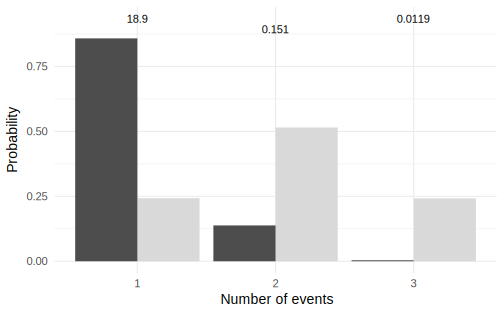
\includegraphics[height=5.4cm]{../../gekko-bake-off/results/dppmsbayes-nevents.pdf}}
}

\bigskip
Run time: 47.3 days
\end{frame}

\begin{frame}
    \frametitle{Caveats}
    \begin{itemize}
        \item We have to make strong prior assumptions about the relative rates
            of mutation among our taxa.

        \bigskip
        \item The model assumes no migration after divergence
    \end{itemize}
\end{frame}


\end{document}
